\documentclass[11pt]{article}
\usepackage[subpreambles=true]{standalone}
\usepackage{acl2012}

\usepackage{latexsym}

\usepackage{newtxtext}
\usepackage[scaled=.90]{helvet}
\usepackage{courier}
%\usepackage{times}

%\usepackage[T1]{fontenc}
%\usepackage{fontspec}
\usepackage{microtype}
\usepackage{flushend}


\usepackage[author={Lyndon White}]{pdfcomment}

\usepackage{verbatim}
\usepackage{grffile}


\usepackage{pgfplots}
\pgfplotsset{compat=1.12}
\usepackage{booktabs, array} % Generates table from .csv
\usepackage{pgfplotstable}


\usepackage{tikz}
\usetikzlibrary{positioning}
\usepackage{xifthen}

%%%%%%%%%%MATH
\usepackage{amsthm}
\usepackage{amsmath}
\usepackage{amssymb}
\usepackage{mathtools}
\usepackage{multirow}

%\usepackage{amsfonts}

\theoremstyle{plain}
\newtheorem{thm}{\protect\theoremname}
\theoremstyle{definition}
\newtheorem{defn}[thm]{\protect\definitionname}
\usepackage{csquotes}
\usepackage[english]{babel}
\providecommand{\definitionname}{Definition}
\providecommand{\theoremname}{Theorem}
%%%%%

%\usepackage[backend=bibtex,
% style=authoryear-icomp,
% bibencoding=ascii,
% maxcitenames=2,
% url=false,
% hyperref=false
%]{biblatex}

%Plain Bibtex way, with the BST
\bibliographystyle{acl2012}
\newcommand{\parencite}{\protect\cite}
\newcommand{\textcite}{\protect\newcite}





\usepackage{cleveref}


%End Packages

%%%%%%%%%%%%%%%%%%%%%% Magic Float Layer Fix Settings 
\renewcommand{\topfraction}{.85}
\renewcommand{\bottomfraction}{.7}
\renewcommand{\textfraction}{.15}
\renewcommand{\floatpagefraction}{.8}
\renewcommand{\dbltopfraction}{.66}
\renewcommand{\dblfloatpagefraction}{.8}
\setcounter{topnumber}{9}
\setcounter{bottomnumber}{9}
\setcounter{totalnumber}{20}
\setcounter{dbltopnumber}{9}

%%%%%%%%%%%%%%%%%




\DeclareMathOperator*{\argmin}{argmin}
%%%%%%%%%% Plots
\newcolumntype{H}{>{\setbox0=\hbox\bgroup}c<{\egroup}@{}}

\pgfplotsset{resplot/.style = {%
		xlabel=Ground Truth Sentence Length,
		xmin=0,xmax=20, xtick={0,2,4,6,8,10,12,14,16,18},
		width=0.95\columnwidth, height=0.8\columnwidth}}


%%%%%%% Tables
\newcolumntype{C}[1]{>{\centering\arraybackslash}m{#1}}

\pgfplotstableset{percent style/.style=}
		}},
		every head row/.style={after row=\midrule},
	}

%%%%%% Data
 
\pgfplotstableread[col sep=comma,ignore chars={"}]{data/ordering_length_scores.csv}{\ordlenscores}
\pgfplotstableread[col sep=comma,ignore chars={"}]{data/ordering_length_scores_oracle.csv}{\ordlenscoresoracle}
\pgfplotstableread[col sep=comma,header=has colnames]{data/selection_len_scores.csv}{\sellenscores}

%%%%%%%%%
%Consistency in naming 
\newcommand{\oracletitle}{Ref.~BOW+Ord.}
\newcommand{\selectiontitle}{Sel.~BOW~Only}
\newcommand{\twosteptitle}{Sel.~BOW+Ord.}

%%%%%%%%

%opening
\title{A \twosteptitle{} Process for Generating Sentences from the Sums of their Embeddings}
\author{}
\graphicspath{{./figs/}}
\setlength\itemsep{2mm}
\begin{document}

\maketitle

\begin{abstract}

	
Converting a sentence to a meaningful vector representation has uses in many NLP tasks, however very few methods allow that representation to be restored to a human readable sentence. Being able to generate sentences from the vector representations is expected to open up many new applications. We introduce such a method for moving from sum of word embedding representations back to the original sentences. This is done using a greedy algorithm to convert the vector to a bag of words. We then show how the bag of words can be ordered using simple probabilistic language models to get back the sentence. To our knowledge this is the first work to demonstrate qualitatively the ability to reproduce text from a large corpus based on its sentence embeddings. 
As well as practical applications for sentence generation, the success of this method has theoretical implications on the degree of information maintained by the sum of embeddings representation.
\end{abstract}

\section{Introduction} \label{intro}
We present a method for generating sentences based on vector representations of the sum of their word embeddings. The generation task, going from any vector representation back to a sentence, is quite challenging. It has not received a lot of attention.

\textcite{Dinu2014CompositionalGeneration} motivates this work from a theoretical perspective given that a sentence encodes its meaning, and the vector encodes the same meaning, then it must be possible to translate in both directions between the natural language and the vector representation. An implementation, such as the work reported in this paper, which demonstrates the truth of this dual space theory has its own value. There are also many potential practical applications of such an implementation, often ranging around certain types of ``translation'' tasks.

There are a number of techniques for learning to associate various media and sentences to a common vector space. Such as  \textcite{farhadi2010every} and \textcite{socherDTRNN} for images; \textcite{KaagebExtractiveSummaristation} and \textcite{yogatamaextractive} for multi-document summaries, and \textcite{zhang2014BRAE} for sentences in multiple languages. However, all of these techniques are tied to being able to use the vector space to compare the sentences and other media for similarities. With appropriate generative models for sentence vectors, these ``matching'' tasks -- that can find the most similar sentence to a vector from a list; become ``generative'' tasks -- that can generate a new sentence.

There are currently three existing methods for sentence regeneration -- each tied to different machine learnt vector representations.
The current state of the art for full sentence generation are the works of \textcite{iyyer2014generating} and \textcite{Bowman2015SmoothGeneration}. 
Both these have been demonstrated to produce full sentences -- advance beyond the original work in the area of \textcite{Dinu2014CompositionalGeneration}. These sentences are qualitatively shown to be loosely similar in meaning to the original sentences. Neither works has produced quantitative evaluation, making it hard to compare their performance. Both are detailed further in the next section.


The two step method proposed in this paper takes in a sum of word embeddings (SOWE) sentence vector, and outputs the sentence which it corresponds to. The input is a vector for example $\tilde{s}=[0.11, 0.57,-0.21,...,1.29]$, which approximates a SOWE vector, and outputs a sentence: for example "The boy was happy.". That input vector could come direct as the SOWE representation of a reference sentence (as is the case for the evaluation presented here). More practically it could come as the output of some other process; for example a machine learnt mapping from an image to the vector representation of its textual description. This vector representation is transformed through our process into a human readable sentence.

Our method performs the sentence generation in two steps, as shown in \Cref{block_diagram}. It combines the work of \textcite{White2015BOWgen} on generating bags of words (BOW) from SOWE (Word Selection); with the work of \textcite{Horvat2014} on ordering BOW into sentences (Word ordering). The overall two step approach can generate proper sentences from SOWE vectors.
\begin{figure}
	\centering 
	\documentclass{standalone}

\usepackage{tikz}
\usetikzlibrary{positioning}


\begin{document}

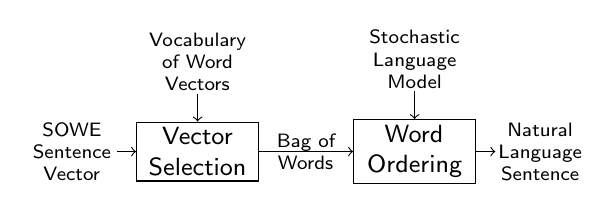
\begin{tikzpicture}[
	every node/.style={ text width=4em,
    					align=center,
                        font=\scriptsize\sffamily,
                        inner sep=1pt
                        },
	proc/.style= {draw,
    			  font=\small\sffamily,
                  inner sep = 2pt
    }
]
	\node (input) [inner sep=-4pt] {SOWE Sentence Vector};
    \node (selection) [proc, right = 0.7em of input]{Vector\\ Selection};
    \node (ordering) [proc, right = 3.4em of selection]{Word\\ Ordering};
	\node (vocab) [above = 1em of selection]{Vocabulary of Word Vectors};
    \node (lm) [above = 1em of ordering] {Stochastic Language Model};
    \node (output) [inner sep=-4pt, right=0.7em of ordering] {Natural Language Sentence};
    \draw[->] (input) -- (selection);
    \draw[->] (vocab) -- (selection);
    \draw[->] (selection) -- (ordering) node[midway] {Bag of Words};
    \draw[->] (lm) -- (ordering);
    \draw[->] (ordering) -- (output);
\end{tikzpicture}

\end{document}
	\caption{The \twosteptitle{} process for the regenerating sentences from SOWE-type sentence vectors.}
	\label{block_diagram}
\end{figure}

The rest of the paper is organized into the following sections. \Cref{relwork} introduces the area, discussing in general sentence models, and prior work on generation. \Cref{framework} explains the problem in detail and how the \twosteptitle{} method is used to solving it. \Cref{evalsettings} describes the settings used for evaluation. \Cref{results} presents the results on this evaluation. The paper concludes with \Cref{conclusion} and a discussion of future work on this problem.


\section{Related Works}\label{relwork}
\subsection{Embedding Models}
There are two general types of embedding methods for sentences: compositional, and non-compositional. 

Compositional modules use a hierarchical  break-down of a sentence into clauses, phrases and words. Compositional models produce embeddings for each component which is then composed (merged) produce the embeddings for its super component and so forth up the syntactic tree. Compositional models include the works of \textcite{Mitchell2008}, \textcite{socher2014recursive} and \textcite{TACL15CompVector}, and in the generative sense \textcite{Dinu2014CompositionalGeneration} and \textcite{iyyer2014generating}. They use the inherent structure of the sentence to produce embeddings. This structure is disregarded by most non-compositional models.

Non-compositional models do not combine substructure embeddings to produce a sentence embeddings. This is a wide and varied class. It includes simple methods like the bag of words (BOW), and the sum of word embeddings (SOWE). It also includes the more advanced methods of \textcite{le2014distributed}, and the generative method of \textcite{Bowman2015SmoothGeneration}. By disregarding structure, there is less indirection in the transfer of information from words vectors to sentence vectors. Even though some information is lost -- e.g. all word order in the case of BOW and SOWE -- overall they can perform better than the compositional models.

Recently the works of \textcite{RitterPosition} and \textcite{White2015SentVecMeaning} found that when classifying sentences into categories according to meaning, simple SOWE outperformed more complex models. Both works used sentence embeddings as the input to classifiers. \textcite{RitterPosition} classified challenging artificial sentences into categories based on the positional relationship described using Na{\"\i}ve Bayes. \textcite{White2015SentVecMeaning} classified real-world sentences into groups of semantically equivalent paraphrases. In both cases, they found the best SOWE-type sentence embeddings to be amongst the highest performing representations. In the case of \textcite{RitterPosition} it outperformed the next best representation by over 5\%. In the case of \textcite{White2015SentVecMeaning} it was within a margin of 1\% from the very best performing method. These results suggest there is a lot of consistency in the relationship between a point in the SOWE space, and the meaning of the sentence. Thus this simple method is worth further consideration. SOWE is the basis of the work presented in this paper.

\subsection{Sentence Generation from Vector Embeddings}

To the best of our knowledge only three prior works exist in the area of sentence generation from embeddings. The first two of which are based on compositional embeddings, while the most recent work at the time of this writing, is based on a non-compositional approach.

\newcommand{\p}{\tilde{p}_{1,2}}
\renewcommand{\u}{\tilde{u}}


\textcite{Dinu2014CompositionalGeneration}  extends the models described by \textcite{zanzotto2010estimating} and \textcite{Guevara2010} for generation. The composition is described as the sum of pair of linear transformations of the input word vectors to get a output vector, and another pair to reverse the composition reconstructing the input. The linear transformation matrices are solved for using least squares. This method of composing, can be applied recursively from words to phrases to clauses and so forth.
It theoretically generalises to whole sentences, by recursive application of the composition or decomposition functions, however in Dinu and Baroni's work is quantitatively assessed only on direct reconstruction for decomposing Preposition-Noun and Adjective-Noun 2 word phrases. In the case where the decomposition function was trained on vectors generated using the compositional function they were able to get perfect reconstruction on the word embedding based inputs.
% -- though as they note, this is not extremely difficult as it is fitting linear transformation to invert a linear transformation.

\renewcommand{\p}{\tilde{p}}

The work of \textcite{iyyer2014generating} extends the work of \textcite{SocherEtAl2011:PoolRAE} defining an unfolding recursive dependency-tree recursive autoencoder (DT-RAE). Recursive neural networks are jointly trained for both composing the sentence's words into a vector, and for decomposing that vector into words. This composition and decomposition is done by reusing a composition neural network at each vertex, the  dependency tree structure with different weight matrices for each dependency relation. The total network is trained based on the accuracy to reproduce its input word vectors, through back-propagation. It can be used to generate sentences, if a dependency tree structure for the output is provided. This method was demonstrated quantitatively on five examples (shown in \Cref{egiyyer}); they found generated sentences to be loosely semantically similar to the originals.

%$$g_{comp}\:: (u_i)^N_{i=1} \mapsto \sigma(\sum_{i=1}^N W_i\u_i+\tilde{b})$$
%$$g_{decomp} \p \mapsto  (\sigma(W^\prime_i\p+\tilde{b}^\prime+W_{sib}\u^\prime_j)^N_{i=1}$$
%$\u^\prime_j$ is $g_{decomp}(p)_j$ if $j$ is the left most sibling of $i$ with the same dependancy relation to the parent as $i$ if one exists, or the zero vector otherwith
%Here $W_i$ and $W^\prime_i$ vary not by order, but by the dependency tree part of speech of the $i$th element.
%$\tilde{b}$ and $\tilde{b}^\prime$ are the biases.
%$\sigma$ is a nonlinear activation function, such as the sigmoid or the hyperbolic tangent functions. It is this nonlinearity that prevents the values being solved by any kind of least squares.

%Theoretically, even without the extensions the unfolding recursive auto-encoder could be used in the same way to generate sentences, however this has not been shown.


\textcite{Bowman2015SmoothGeneration} uses a a modification of the variational autoencoder (VAE) \parencite{kingma2013auto} with natural language inputs and outputs, to learn the sentence representations. These input and output stages are performed using long short-term memory recurrent neural networks \parencite{hochreiter1997long}. They demonstrate a number of uses of this technique, only one of which is sentence generation, in the sense of this paper.
While it is a generative model it does not seek to recreate a sentence purely from its vector input, but rather to produce a series of probability distributions on the words in the sentence. These distributions can be evaluated greedily, which the authors used to give three quantitative examples of resynthesis (also shown in \Cref{egbowman}). They found the sentence embeddings created were storing largely syntactic and loose topical information. 

None of the existing methods have demonstrated recreation of the full sentence input close enough to allow for quantitative evaluation on a full corpus. They tend to output lose paraphrases, or roughly similar sentences -- itself a separately useful achievement.  That is not the case for our method described in the next section, which can often exactly recreate the original sentence from its vector representation.

Unlike current sentence generation methods, the BOW generation method of \textcite{White2015BOWgen} generally outputs a BOW very close to the reference for that sentence -- albeit at the cost of loosing all word order information. It is because of this accuracy that we base our method on it (as detailed in \Cref{selection}). The Word Selection step we used is directly based on their greedy BOW generation method. We improve it for sentence generation by composing with a word ordering step to create the two step sentence generation process.


\section{General Framework: \twosteptitle{} Generation}\label{framework}
As discussed in \Cref{intro}, and shown in \Cref{block_diagram}, the approach taken to generate the sentences from the vectors comes in two steps. First selecting the words used -- this is done deterministically, based on a search of the embedding space. Second is to order them, which we solve by finding the most likely sequence according to a stochastic language model. The separating of the process into two steps is unlike any of the existing methods for sentence generation from vectors. The two subproblems which result from this split resemble more classical NP-Hard computer science problems; thus variations on known techniques can be used to solve them.
% The selection problem, of choosing the word vectors to sum be closest to the target is a knapsack-like problem. The word-ordering problem is a search for the most-likely path through a Markov graph of n-gram probabilities -- a variation on the travelling salesman problem. It may be noted, that both these sub-problems are NP-hard.


\subsection{Word Selection} \label{selection}
\renewcommand{\c}{\tilde{c}}
\newcommand{\s}{\tilde{s}}
\newcommand{\x}{\tilde{x}}
\renewcommand{\t}{\tilde{t}}
\newcommand{\N}{\mathbb{N}}
\newcommand{\R}{\mathbb{R}}
\newcommand{\V}{\mathcal{V}}
\def\B{\mathcal{B}}




\textcite{White2015BOWgen} solves the BOW generation problem, by solving what they call the vector selection problem -- selecting the vectors that sum up closest to a given vectors. This is related to the knapsack and subset sum problems. They formally define the vector selection problem as:
\[
(\s,\V,\,d) \mapsto \argmin_{\left\{ \forall\c\in\N_{0}^{V}\right\} }\:d( \s,\,\sum_{\x_j\in\V}\:\x_{j}c_{j})
\]
to find the bag of vectors selected from the vocabulary set $\V$ which when summed is closest to the target vector $\s$. Closeness is assessed with distance metric $d$. $\c$ is the indicator function for that multi-set of vectors. As there is a one to one correspondence between word embeddings and their words, finding the vectors results in finding the words. \textcite{White2015BOWgen} propose a greedy solution to the problem.

The key approach proposed by \textcite{White2015BOWgen} is greedy addition. The idea is to greedy add vectors to a partial solution building towards a complete bag. This starts with an empty bag of word embeddings, and at each step the embedding space is searched for the vector which when added to the current partial solution results in the minimal distance to the target -- when compared to other vectors from the vocabulary. This step is repeated until there are no vectors in the vocabulary that can be added without moving away from the solution. Then a fine-tuning step, n-substitution, is used to avoid some simpler greedy mistakes.

The n-substitution method avoids mistakes by examining partial solutions (bags of vectors) and seeing if it is possible to find a better solution by removing n elements and replacing them with up-to n different elements. The replacement search is exhaustive over the n-ary cartesian product of the vocabulary. Only for $n=1$ is it currently feasible for practical implementation outside of highly restricted vocabularies. Never-the-less even 1-substitution can be seen as lessening the greed of the algorithm, through allowing early decisions to be reconsidered in the full context of the partial solution. The algorithm does remain greedy, but many simple mistakes are avoided by n-substitution. The greedy addition and n-substitution processes are repeated until the solution converges.



\subsection{The Ordering Problem} \label{ordering}
\begin{figure*}
	\begin{center}
	\documentclass{standalone}
\usepackage{arrayjobx}
\usepackage{xifthen}
\usepackage{tikz,textcomp}
\usepackage{ amssymb }

\begin{document}
	
\tikzset{ shorten <>/.style={ shorten >=0.2cm, shorten <=0.2cm } }

\begin{tikzpicture}
\newarray\Words
\readarray{Words}{$w_\triangleright$&$w_1$&$w_2$&$w_3$&$w_4$&$w_\triangleleft$}
\dataheight=5

\newcommand{\ystep}{0.5}

\newcommand{\gx}{}
\newcommand{\gy}{}


\newcommand{\drawgroupinner}{
	\foreach \j in {1,...,6}
	{
		\colorlet{MyColor}{black}%
		\ifthenelse{\i=\j}{\colorlet{MyColor}{gray}}{}
		\ifthenelse{\j=1}{\colorlet{MyColor}{gray}}{}
		
		\node[MyColor] (w_\i\j) at (\gx,\gy-\ystep*\j cm) {\Words(\i)\Words(\j)};
	}
	\draw (\gx,\gy-3.5*\ystep cm) ellipse (0.7cm and \ystep*4 cm);
}

\newcommand{\drawgrouptop}[3]{%
	\renewcommand{\i}{#1}
	\renewcommand{\gx}{#2 cm}
	\renewcommand{\gy}{#3 cm}
	\drawgroupinner{}	
	\node at (\gx,\gy+1*\ystep cm) {$S($\Words(\i)$)$};

}
\newcommand{\drawgroupbottom}[3]{%
	\renewcommand{\i}{#1}
	\renewcommand{\gx}{#2 cm}
	\renewcommand{\gy}{#3 cm}
	\drawgroupinner{}	
	\node at (\gx,\gy-8*\ystep cm) {$S($\Words(\i)$)$};	
}



\drawgrouptop{1}{0}{0}
\drawgrouptop{2}{2.5}{2.5}
\drawgroupbottom{3}{5}{-1.5}
\drawgrouptop{4}{7.5}{2.5}
\drawgrouptop{5}{10}{0}



\foreach \i in {1,...,5}
{	
	\foreach \j in {2,...,5}
	{
		\colorlet{MyColor}{black}%
		\ifthenelse{\j=2}{\colorlet{MyColor}{cyan!50!black}}
		{\ifthenelse{\j=3}{\colorlet{MyColor}{blue!50!black}}%
%		{\ifthenelse{\j=3}{\colorlet{MyColor}{red!50!black}}%
		{\ifthenelse{\j=4}{\colorlet{MyColor}{yellow!50!black}}%
		{\ifthenelse{\j=5}{\colorlet{MyColor}{green!50!black}}%
		{}}}}%}


		\ifthenelse{ \NOT \i=\j}{
			\foreach \k in {2,...,6}
			{
				\ifthenelse{\NOT \k=\i \AND \NOT \k=\j}
				{
					\draw[->,MyColor] (w_\i\j) -- (w_\j\k);
				}{}
			}
		}{}
	}
}

\node (w_S) at (-2cm,-1.5) {$w_\blacktriangleright$\Words(1)};
\draw (-2cm,-1.5) ellipse (0.7cm and 1 cm);
\node at (-2cm,-1.5cm +1.3 cm) {$S(w_\blacktriangleright)$};


\foreach \j in {2,...,5}
{
	\draw[->, red!70!black] (w_S)  --  (w_1\j);
}


\node (w_E) at (12cm,-1.5) {\Words(6)$w_\blacktriangleleft$};
\draw (12cm,-1.5) ellipse (0.7cm and 1 cm);
\node at (12cm,-1.5cm +1.3 cm) {$S($\Words(6)$)$};
\foreach \j in {1,...,5}
{
	\draw[->, red!70!black] (w_\j6) -- (w_E);
}

%\draw[->,line width=1mm,brown] (w_S) -- (w_12) -- (w_23)--(w_34)--(w_45)--(w_56)--(w_E);

\end{tikzpicture}

\end{document}
	\end{center}
	\caption{\label{fig:ordergraph} A graph showing the legal transitions between states, when the word-ordering problem is expressed similar to a GA-TSP. Each edge $(w_aw_b)\to (w_bw_c)$ has cost $-\log(P(w_c\:|\:w_aw_b)$. The nodes are grouped into columns for each district (word). In bold is shown one legal path which goes from beginning, to end, and covers all districts (words).} 
\end{figure*}

After the bag of words has been generated by the previous step, it must be ordered. For example ``are how , today hello ? you'', is to be ordered into the sentence: ``hello , how are you today ?''. This problem can not always be solved to a single correct solution. \textcite{Mitchell2008}  gives the example of "It was not the sales manager who hit the bottle that day, but the office worker with the serious drinking problem." which has the same word content (though not punctuation) as "That day the office manager, who was drinking, hit the problem sales worker with a bottle, but it was not serious.". However, while a unique ordering can not be guaranteed, finding the most likely word ordering is possible.

\textcite{Horvat2014} formulated the word ordering problem an a generalised asymmetrical travelling salesman problem (GA-TSP). \Cref{fig:ordergraph} shows an example of the connected graph for ordering five words. We extend beyond the approach of \textcite{Horvat2014} by reformulated the problem as a linear mixed integer programming problem (MIP). This lets us take advantage of the efficient existing solvers for this problem. 
Beyond the GA-TSP approach, direct MIP formulation allows for increased descriptive flexibility and opens the way for further enhancement. The description is freed of some of the constraints of a TSP. For example, word ordering does have distinct and known start and end nodes (as shall be detailed in the next section). To formulate it as a GA-TSP it must be a tour without beginning or end. \textcite{Horvat2014} solve this by simply connecting the start to the end with a zero cost link. This is not needed if formulating this as a MIP problem, the start and end nodes can be treated as a special case. Being able to special case them as nodes known always to occur allows some simplification in the subtour elimination step. The formulation to mixed integer programming is otherwise reasonably standard.



\documentclass[twocolumn]{article}
%\documentclass{standalone}
\usepackage{verbatim}
\usepackage{amsthm}
\usepackage{amsmath}
\usepackage{amssymb}
\usepackage{mathtools}
\usepackage{multirow}

\begin{document}
\newcommand{\s}{w_{\blacktriangleright}}
\renewcommand{\ss}{w_{\triangleright}}
\newcommand{\e}{w_{\triangleleft}}
\newcommand{\ee}{w_{\blacktriangleleft}}
\newcommand{\W}{\mathcal{W}}


\subsubsection{Notation}

The following notion is used:

For $\W$ the bag of words to be ordered, including the start ($\s$,$\ss$)
and end pseudo-words.($\e$, $\ee$)

We will write $w_{i}\in\W$ to represent a word from the bag, with
arbitrarily assigned subscripts. Where a word occurs with multiplicity
greater than 1, it is assigned multiple subscripts, and each is treated
as a distinct word.

Each vertex is a sequence of two words, $\langle w_{i},w_{j}\rangle\in\W^{2}$.
This is a Markov state, consisting of a word and its predecessor word. \\
Each edge between two vertices represents a transition from one trigram state to another.
The Start vertex is given by $\langle\s,\ss\rangle$, and the end by $\langle\e,\ee\rangle$.

The GA-TSP districts are given by the sets of all states that have
a given word in the second position. The district for word $w_{j}$
is given by $S(w_{j})\subseteq\W^{2}$, defined as $S(w_{j})=\{\langle w_{i},w_{j}\rangle\,\mid\,w_{i}\ne w_{j}\,\wedge w_{i}\in\W\}$. It is required to visit every district, thus it is required to use every word.




\subsubsection{Optimization Model}

The path and its costs are modelled by:

A transition from $\langle w_{i},w_{j}\rangle$ to $\langle w_{j},w_{k}\rangle$
transitions has cost $$C[\langle w_{i},w_{j}\rangle,\langle w_{j},w_{k}\rangle]=-\log\left(P(w_{k}|w_{i},w_{j}\rangle\right)$$ 
The table of transitions to be optimized is
\begin{multline*}
 \tau[\langle w_{a},w_{b}\rangle,\,\langle w_{c},w_{d}\rangle] = \\
 \begin{cases}
	 \multirow{3}{*}{1} & \mathrm{if\,transition\,from} \\
	 	                & \langle w_{a},w_{b}\rangle \to \langle w_{c},w_{d}\rangle\\
	 	                & \mathrm{occurs} \\
                     0  & \mathrm{otherwise}
  \end{cases}
\end{multline*}

The total cost to be minimized, is given by
\begin{multline*}
 C_{total}(\tau)= \\
	 \sum_{\mathrlap{\!\!\!\!\forall\left[\langle w_{a},w_{b}\rangle,\langle w_{c},w_{d}\rangle\right]\in\left(\W^{2}\right)^{2}
 	}}
 	\;\tau[\langle w_{a},w_{b}\rangle,\,\langle w_{c},w_{d}\rangle] \cdot C[\langle w_{a},w_{b}\rangle,\,\langle w_{c},w_{d}\rangle]
\end{multline*}

\begin{comment}
\begin{multline*}
C_{total}(\tau)= 
\sum_{\mathclap{
		\left[w_{ab},w_{cd}\right]\in\left(\W^{2}\right)^{2}
	}}
	\;\tau[w_{ab},w_{cd}] \cdot C[w_{ab},w_{cd}]
\end{multline*}
\end{comment}

The probability of a particular path (i.e. of a particular ordering)
is thus given by 
\begin{equation*}
P(\tau)=e^{-C_{total}(\tau)}
\end{equation*}

The word order can be found by following the links. The function 
$f(n,\tau)$ gives the word that, according to $\tau$ occurs in the $n$th position.

\begin{multline*}
f(n,\tau)= \\
\begin{cases}
\{w_{a}\mid\tau[\langle\s,\ss\rangle,\langle\ss,w_{a}\rangle]=1\}_{1} & n=1\\
\{w_{b}\mid\tau[\langle\ss,f(1,\tau)\rangle,\langle f(1,\tau),w_{b}\rangle]=1\}_{1} & n=2\\
\{w_{c}\mid\tau[\langle f(n{-}2,\tau),f(n{-}1,\tau)\rangle,\langle f(n{-}1,\tau),w_{c}\rangle]=1\}_{1} & n\ge3
\end{cases}
\end{multline*}

%\pdfcomment{I think maybe the overlarge equation is best replaced with some kind of wordy description}

Note that if $\tau$ follows the constraints that follow then valid then, then
each set is a singleton, $\{\}_{1}$ indicates taking the singleton set's only element.




\subsubsection{Constraints}

The requirements of the problem, place various constraints on to $\tau$:

The Markov state must be maintained: $\forall\langle w_{a},w_{b}\rangle,\langle w_{c},w_{b}\rangle\in\W^{2}$:
\begin{equation*}
w_{b}\ne w_{c} \implies \tau[\langle w_{a},w_{b}\rangle,\,\langle w_{c},w_{d}\rangle]=0
\end{equation*}

Every node entered must also be left -- except those at the beginning and end.
\begin{multline*}
\forall\langle w_{i},w_{j}\rangle\in\W^{2}\backslash\{\langle\s,\ss\rangle,\langle\e,\ee\rangle\}: \\
 \sum_{\mathrlap{\!\!\!\!\forall\langle w_{a},w_{b}\rangle\in\W^{2}}}\tau[\langle w_{a},w_{b}\rangle,\,\langle w_{i},w_{j}\rangle]
=\sum_{\mathrlap{\!\!\!\!\forall\langle w_{c},w_{d}\rangle\in\W^{2}}}\tau[\langle w_{i},w_{j}\rangle,\,\langle w_{c},w_{d}\rangle]
\end{multline*}

Visit (enter) every district exactly once. i.e. use every word exactly once.
\begin{multline*}
\forall w_{j}\in\W\backslash\{\s,\ss\}: \\
\sum_{\mathclap{\forall\langle w_{i},w_{j}\rangle\in S(w_{j}\rangle}}
\sum_{\mathclap{\substack{\; \\ \;\\ \forall\langle w_{a},w_{b}\rangle\in\W^{2}}}}
\tau[\langle w_{a},w_{b}\rangle,\,\langle w_{i},w_{j}\rangle]=1
\end{multline*}

To allow the feasibility checker to detect if ordering the words is
impossible, transitions of zero probability are also forbidden. i.e. if
$P(w_{n}|w_{n-2},w_{n-1})=0$ then $\tau[\langle w_{n-2},w_{n-1}\rangle,\langle w_{n-1},w_{n}\rangle]=0$.
These transitions, if not expressly forbidden, would never occur in
an optimal solution in any case, as they have infinitely high cost.


\paragraph{Lazy Subtour Elimination Constraints}

The problem as formulated above can be input into the MIPS solver. However, like similar formulation of the
travelling salesman problem, some some solutions will have subtours.
We take the usual method for handling this an use callbacks to impose
lazy constraints to forbid such solutions at run-time.  
However the actual formulation of those constraints are different to a typical GA-TSP.

Given a potential solution $\tau$ meeting all other constraints:
\begin{itemize}
\item The core path -- which starts at the beginning $\langle\s,\ss\rangle$
and ends at $\langle\e,\ee\rangle$the end can be found. This is done
by practically following the links from the start node, and accumulating
them into a set $T\subseteq\W^{2}$
\item From the core path, the set of words covered is given by $\W_{T}=\{w_{i}\,\mid\,\forall\langle w_{i},w_{j}\rangle\in T\,\}\cup\{\ee\}$.
If $\mathcal{W_{T}}=\W$ then there are no subtours and the core-path
is the full. Otherwise, there is a subtour to be eliminated.
\item If there is a subtour, then to eliminate it, a constraint must be
added. This constraint is that there must be a connection from at
least one of the nodes in the district covered by the core path to
one of the nodes in the districts not covered.
\item The districts covered by the tour are given by $S_{T}=\bigcup_{w_{t}\in W_{T}}S(w_{t})$,
\item subtour elimination constraint is given by 
\begin{equation*}
  \sum_{\mathclap{\forall\langle w_{t1},w_{t2}\rangle\in S_{T}}}
  \sum_{\mathclap{\substack{\; \\ \;\\ \forall\langle w_{a},w_{b}\rangle\in\W^{2}\backslash S_{T}}}}
  \tau[\langle w_{t1},w_{t2}\rangle,\langle w_{a},w_{b}\rangle]\ge1
\end{equation*}
\item i.e. There must be a transition from one of the states featuring a
word that is in the core path, to one of the states featuring a word
not converted by the core path.

\end{itemize}
It is the formulation around the notion of a core-path that differs this from typical subtour elimination in a GA-TSP. True GA-TSP problems are not guaranteed to have any nodes which must occur. However every word ordering problem is guaranteed to have such a node -- the start and end nodes. This thus makes it possible to identify what is generally the path that requires the least modification to get to a complete solution, as the path to require changes on. Other heuristics, and subtour elimination constraints do exist however.


\end{document}


\begin{comment}
Each word in the BOW is ascribed an arbitrary index. For words occurring with multiplicity greater than 1, they are ascribed multiple indices, and treated as per differing words. The sentences are supplemented with pseudowords, with two placed a the beginning  and end of the sentences. These pseudowords allow the trigram language model to indicate information about the words which occur near the sentence boundaries. We then use the language model's word subsequence probabilities to express the problem as a graph.

The word-ordering problem is expressed as a GA-TSP, by mapping trigram states, to nodes, transition probabilities to edge costs, and words to districts. A diagram for the ordering of a BOW of size five is shown in \Cref{fig:ordergraph}. Each node corresponds to a pair of words, corresponding to the previous two words before the edge. This includes the pseudowords used at the start ( $w_\triangleright$ and $w_\blacktriangleright$) and end ($w_\triangleleft$ and $w_\blacktriangleleft$) which are the initial and terminal nodes. This is the Markov state for the trigram language model. Each edge is a transition between these states and has cost given by the language model. $w_aw_b\to w_bw_c$ has cost given by $-\log(P(w_c\:|\:w_aw_b)$. Each district, is a group of nodes sharing a common word in the second first position (it could be defined equivalently with districts from second position). Every district must be visited exactly once, this is one of the constants on the optimisation problem.

The districts constraint is the defining difference of the generalised TSP. It is sometime for this reason known as the Neighbourhood TSP, the Multiple Choice TSP, the Covering Salemans Problem and the One-of-a-Set TSP \parencite{Gudmundsson1999}. In this case the districts correspond to having a word in the state. Every word ($w_i$), must be used once. This means the for district two shown in \Cref{fig:ordergraph}, one of the nodes: ${w_2w_\triangleright, w_2w_w,w_2w_3,w_2w_4, w_2w_5, w_2,w_\triangleleft}$ must be visited. It those these districts are not spatially located -- we are not working with TSP in the plane, but over a non-complete directed graph.

The connections between nodes, are constrained to ensure consistency of the Markov state. As the second element of the state is the word before the transition, and the first element the word before that, then the state transitioned to must maintain that state. For example no edge can exist between $w_2w_3$ and $w_4w_5$, but one could exist between $w_2w_3$ and $w_3w_5$. Similar to the Markov consistency constraint is the path constraint.

%This is a form of enhanced state, to ensure the assumed Markov property that the next state (i.e. the legal transition) probability depends only previous state -- i.e. the next word depends only on previous two words.

The key constraint on the path is that every node entered, must be exited. For example as if there is the transition $w_1w_2 \to w_2w_3$ then having a transition $w_2w_4\to w_4w_5$ would not be allowed, as that would have a "jump" within the district  of $w_2$ -- which is not a continuous path. The exception to this is the end node ($w_\triangleleft w_\blacktriangleleft$), which does not have to be exited. This can be expressed in MIP form as saying the number of edges entering a node (zero or one) is equal to the number of edges leaving the node (zero or one).

Once the problem is expressed as a GA-TSP we went on to express the problem further into a MIP form. This meant the use of a generalised a MIP solver, rather than the TSP solver used by \textcite{Horvat2014}. Reducing the problem to a linear mixed integer programming problem is a very common technique to solve TSP-like problems. We followed a fairly standard formulation \pdfcomment{Should I give equations here?}. This direct expression allowed us to vary the problem, with the potential for small optimisations. 


Normally, for a problem with known start and end vertices to be considered as a travelling salesman problem, the vertices are connected with a zero cost link. As there are exactly one Start and End pseudo-word states we simply special case them in the MIP definition as not requiring incoming or outgoing connections, respectively. We also made direct use of the knowledge that the Start and End states must to always occur in every tour, to simplify the sub-tour elimination. 

When the travelling salesman problem is solved as a MIP,  some potential solutions contain non-connected subtours. These are eliminated by adding new "lazy" constraints are added, each time such a solution is suggested. For the normal TSP, subtours are eliminated with the constraint that every subtour must have an additional outgoing connection to one of the other subtours. This is more complex in case of the generalised asymmetrical TSP: for each subtour there must an outgoing connection from the nodes of the neighbours covered by it, to one of the nodes in the union of the neighbourhoods covered by the other subtours. Finding these unions takes a non-negligible amount of time; but only one of them is needed to eliminate this subtour. When multiple subtours are common adding multiple constraints cause more to be eliminated; however we've found that subtours are rare in the word ordering problems, and multiple subtours even more so -- as such, pre-emptively adding constraints to eliminate them is not efficient computationally. We can quickly find the core tour, by following the path from the Start to the End pseudo-word states. Then we add only the requirement that there is an outgoing connection from the nodes in neighbourhoods covered by the core tour, to one or more of the nodes outside that set. Preliminary testing found this to give a marginal (~10\%) speed-up.

In going forward, expressing the problem directly as a MIP rather than a GA-TSP opens several avenues. It is simple to get the second, third and so forth best solution, by adding a standard MIPs constraint to disallow the better solutions. It also is open to relaxation of constraints. 

When the constraints on the MIP problem render no solution feasible, this prevent an solution being found. For example, there is no possible ordering of most BOW that do not contain a period, question mark, or exclamation mark, most tokens other than these have a zero probability of appearing at the end of the sentence. Adjustments can be made to the MIPs model to detect the cause of the infeasibility (using irreducible inconsistent subsystem methods), and them apply suitable constraint relaxations.




We first formulate the problem into a Markov graph of states (each correspond to potential subsequences of two words), with edges weighted according to the log of the trigram possibility of the transitions between them 

The probability of any sequence of words can be found using a trigram language model. We can express all possible orderings as a graph between Markov states of the last two words, connected to allowable following words by edged weighted by the negative log of the trigram probability. 
 with edges weighted with the logThis language model can be used to 


The problem for ordering is assign an map between 

The problem can be expressed in terms of a Markov  chain
In this section a demonstration of the feasibly of solving for the correct word order, given the output of the previous step is shown. This is a stochastic language modelling problem -- to determine the most likely sequence of words, given the constraints that the words are exactly those given by the BOW output from the previous step. The method presented here is simply to show its feasibility; the development of efficient technique for use in the ordering problem is left for future work.\pdfcomment{LW: I think this sentence/paragraph can be cut down a lot. RT: I agree, If this is a standard approach (used in ASR?) is there a need to describe the background of the beam seach using tri-gram models. YOu should just state what you implemented (with reference of where the beam search using trigrams is used), provide the parameter details in Section 4 and perhaps move the computational analysis (of all compoenents) into a separate section.}

For purposes of this demonstration a simple Kneser-Ney smoothed trigram model \parencite{kneser1995improved} was used. The language model allows us to evaluate the probability of any given sequence of words using a Markov model.
A directed acyclic graph of states can be produced for possible sequences of words as shown in \Cref{markov_diagram}. The graph is restricted, in that terminal nodes must be followed by the end state, and must also have no words from the input BOW unassigned. The task is then modelled as finding the most-likely path through the graph.
Beam search was used to search the graph. At each node in the graph only the beam width most likely transitions, using just the a signal step of the trigram as the heuristic, were considered. This search is not complete, nor optimal -- there may be a better ordering that requires a transition that is outside the beam width. The beam-width restriction allows the combinatorial problem to be completed in feasible time. For a BOW with $n$ words, and beam width $b$ (assuming $b<n$) the time complexity is $O(b^{n-b}b!)$, rather than $O(n!)$ for a full search of all possible orderings. Memorization is also used to avoid re-searching known branches; and branches cease to be  if their accumulated probability for the path becomes zero -- potentially due to underflow on the 64-bit IEEE floating point numbers.

Even with these techniques to decrease the time taken, running the search over long sentences takes significant amount of time: on the order of 10 seconds for a sentence with 18 words, and increasing rapidly. For this reason the ordering step is only carried out for the BOWs corresponding to reference sentences with no more than 18 words.
 
  
Of course, for some sentences the BOW can not always be resolved to the correct ordering -- when some words can be swapped in position and still have a valid and likely sentence. For example ``Show me flights from London to New York.'' is just as reasonable as  ``Show me flights from New York to London.''. On the other hand often one ordering is far more likely and reasonable than the others, "The dog chased the cat." is much more often correct than "The cat chased the dog.", it is also preferable over "The cat the dog chased." though all three are grammatically correct. It is assumed here that, for most bags of words there is one ordering that is far far more likely to occur than the others, and thus is the correct ordering. The results for the Oracle BOW in the next section suggest this assumption is largely correct -- at least for the Brown Corpus.

%\pdfcomment{The next paragraph would benefit from being merged into the former. Or perhaps being made a footnote? Or deleted}
%\textcite{Mitchell2008} gives  example of  "It was not the sales manager who  hit  the bottle that day, but the office worker with the serious drinking problem." and "That day the office manager,   who was drinking, hit the problem sales worker with a bottle, but it was not serious.". It  can be argued that this example is synthetic and that more natural phrasing would have resulted in sentences with different wordings. A second issue is the differing numbers if commas in the texts. Though certainly some sentenced where this is not true must exist, work with the assumption they are rare.
\end{comment}



\section{Experimental Setup and Evaluations} \label{evalsettings}
This experimental data used in this evaluation was
obtained from the data released with \textcite{White2015BOWgen}. \pdfcomment{Need to add link here}
\subsection{Word Embeddings}
GloVe representations of words are used in our evaluations \parencite{pennington2014glove}. There are many varieties of word embeddings which function with our algorithm. GloVe was chosen become of the availability of a large pre-trained vocabulary of vectors. The representations used for evaluation were pretrained on 2014 Wikipedia and Gigaword 5\footnote{Available online at \url{http://nlp.stanford.edu/projects/glove/}}.  Other vector representations are presumed to function similarly.

\subsection{Corpus and Language Modelling}
\begin{figure}
	\centering
	\begin{tikzpicture}
	\begin{axis}[resplot,
	ybar, ymin=0, ytick={0,1000,2000, 3000,4000,5000},
	bar width=1,
	ylabel=Number of Sentences,
	]
	\addplot table [y=Instances,x=ground_length]{\ordlenscores};
	
	\end{axis}
	\end{tikzpicture}
	\caption{\label{fig:corpus} The distribution of the evaluation corpus after preprocessing.}
\end{figure}

The evaluation was performed on a subset of the Books Corpus \parencite{moviebook}. The corpus was preprocessed as per in the work of \textcite{White2015BOWgen}. This meant removing any sentences which used words not found in the embedding vocabulary.

After preprocessing, the base corpus, was split 90:10. 90\% (59,694,016 sentences) of the corpus was used to fit a trigram model. This trigram language model was smoothed with Knesler-Ney back-off \parencite{kneser1995improved}. The remaining 10\% of the corpus was kept in reserve. From the 10\%, 1\% (66,464 sentences) were taken for testing. From this any sentences with length over 18 words were discarded -- the time taken to evaluated longer sentences is too long to be feasible. This left a final test set of 53,055 sentences. \Cref{fig:corpus} shows the distribution of the evaluation corpus in terms of sentence length.
 
Note that the Books corpus contains many duplicate common sentences, as well as many duplicate books: according to the distribution site \footnote{\url{http://www.cs.toronto.edu/~mbweb/}} only 7,087 out of 11,038 original books in the corpus are unique. We did not remove any further duplicates, which means there is a strong chance of a small overlap between the test set, and the set used to fit the trigrams.
 

\subsection{Mixed Integer Programming}
During evaluation we used Gurobi MIP solver version 6.5.0. During preliminary testing we found Gurobi to be significantly faster than the open source GLTK. Particularly for longer sentences, we found two orders of magnitude difference in speed for sentences of length 18. This is inline with the more extensive evaluations of \textcite{meindl2012analysis}. It was run under default settings, other than being restricted to a single thread. Restricting the solver to a single thread allowed for parallel processing.

Processing was carried out on a 12 core AMD Opteron 6300 virtual machine with 45Gb of RAM. Implementation was done in the Julia programming language \parencite{Julia}. The MIP solver was invoked though the JuMP library \parencite{jump}. The implementation, and non-summarised results are available for download online.\footnote{[[URL Blinded for Review]]}



\section{Results and Discussion} \label{results}


\begin{table}	
	\centering
	\resizebox{\linewidth}{!}{
		\setlength{\tabcolsep}{3pt}
		\pgfplotstabletypeset[skip rows between index={0}{4},
		col sep=comma,fixed zerofill, precision=3,column type=C{4em},
		columns/Portion Perfect/.style={percent style, precision=1},
		every head row/.style={after row=\midrule},
		create on use/Process/.style={create col/set list={0,0,0,0,Word Selection}},
		columns/Process/.style = {string type,column type=C{6.5em}},
		%columns={Process, [index]2,[index]3,[index]4,[index]5,[index]6}
		columns={Process, Portion Perfect, Mean Precision,Mean Jaccard Score}
		]{data/selection_overall_len_scores.csv}
	}
	\caption{ The performance of the word selection step, on the Books corpus. Note that the performance of the word selection step, bounds the overall performance shown in \Cref{table:overall}. This table shows a subset of the results reported by \textcite{White2015BOWgen}.}
	\label{table:wordselection}
\end{table}

\begin{table}[t]
	\centering
	\resizebox{\linewidth}{!}{
		\setlength{\tabcolsep}{3pt}
		\pgfplotstabletypeset[col sep=comma, ignore chars={"}, fixed zerofill, precision=3,column type=C{4em},
		columns/Process/.style={string type,column type=C{6.5em}},
		columns/Portion Perfect/.style={percent style, precision=1},
		columns/Portion Perfect (Feasible Only)/.style={percent style, precision=1},
		columns/Portion Feasible/.style={percent style, precision=1},
		every head row/.style={
			after row=\midrule
		},
		columns={Process, Portion Perfect, BLEU Score, Portion Feasible}
		]{data/ordering_scores.csv}}
	\caption{The overall performance of the \twosteptitle{} sentence generation process when evaluated on the Books corpus. The Input column indicates whether the bag of words input to the ordering step was generated using the word selection process, or if it was provided an by an Oracle word sector. }
	\label{table:overall}
\end{table}


\begin{figure}
	\centering
	%\pgfplotstablecreatecol[copy column from table={\sellenscores}{books_0_01_glove300_precision_mean}] {select error} {\ordlenscoresoracle}
	\begin{tikzpicture}
		\begin{axis}[
			resplot,
			legend style={at={(0.02,0.02)},anchor=south west},	
			ylabel=BLEU Score,
			cycle list name=exotic]
		\addplot table [y=BLEU Score,x=ground_length]{\ordlenscores};
		\addplot table [y=BLEU Score,x=ground_length]{\ordlenscoresoracle};
		%\addplot table [y expr=\thisrow{BLEU Score} - (1-\thisrow{select error})
		%	,x=ground_length]{\ordlenscoresoracle};
		
		%\addplot table [y=books_0_01_glove300_precision_mean,x=ground_len]{\sellenscores};
		\legend{\twosteptitle{} , \oracletitle{}}
		\end{axis}
	\end{tikzpicture}
	\caption{\label{figure:bleulenscore} the BLEU score of the entire two step process, vs just the ordering step (with reference BOW).}
\end{figure}


\begin{figure}
	\centering
	\pgfplotstablecreatecol[copy column from table={\sellenscores}{books_0_01_glove300_perfect_mean}] {select error} {\ordlenscoresoracle}
	\begin{tikzpicture}
	\begin{axis}[resplot,
	legend style={at={(0.02,0.02)},anchor=south west},
	xmin=0,xmax=20, xtick={0,2,4,6,8,10,12,14,16,18},
	ylabel=Portion Perfect,
	cycle list name=exotic]
	\addplot table [y=Portion Perfect,x=ground_length]{\ordlenscores};
	\addplot table [y=Portion Perfect,x=ground_length]{\ordlenscoresoracle};
	\addplot[mark=triangle*] table [y=books_0_01_glove300_perfect_mean ,x=ground_len,
					skip coords between index={18}{1000}, 		
	]{\sellenscores};
	
	\legend{\twosteptitle{} , \oracletitle{}, Sel. BOW. Only}
	\end{axis}
	\end{tikzpicture}
	\caption{The portion of sentences reconstructed perfectly by the \twosteptitle{} process. Shown also is the results on ordering only, which orders the reference BOWS, and the results from the Word Selection Step only (the input to the ordering step).}
	\label{figure:exactlenscore}
\end{figure}


\documentclass[class=article]{standalone}
%documentclass{article}
\usepackage{pifont}% http://ctan.org/pkg/pifont
\newcommand{\cmark}{\ding{51}}%
\newcommand{\xmark}{\ding{55}}%\\
\newcommand{\namark}{\ding{54}}
\newcommand{\passmark}{--}
\newcolumntype{C}[1]{>{\centering\arraybackslash}m{#1}}


\usepackage{acl2012}

\begin{document}
	\newcommand{\collenone}{2.3cm}
	\newcommand{\collentwo}{11.5cm}
	\newcommand{\collenthree}{0.5cm}
	\newcommand{\reftitle}{Reference}
	\newcommand{\iref}{DT-RAE Ref.}
	\newcommand{\ip}{DT-RAE Para.}
	\newcommand{\bm}{VAE Mean}
	\newcommand{\bs}{VAE Sample}
	\begin{table*}
		\small
		\begin{tabular}{ p{\collenone} p{\collentwo} C{\collenthree} C{\collenthree} }
			
			\textbf{3A \hfill \reftitle}  & name this 1922 novel about leopold bloom written by james joyce . & \textbf{Sel.} & \textbf{Ord.} \\
			\textbf{\oracletitle}  & written by name this . novel about 1922 bloom leopold james joyce & \passmark & \namark \\
			\textbf{\twosteptitle}  & written novel by name james about leopold this bloom 1922 joyce . & \cmark & \namark \\
			\textbf{\iref}  & name this 1906 novel about gottlieb\_fecknoe inspired by james\_joyce &  &  \\
			\textbf{\ip}  & what is this william golding novel by its written writer &  &  \\
			\hline
			\textbf{3B \hfill \reftitle}  & ralph waldo emerson dismissed this poet as the jingle man and james russell lowell called him three-fifths genius and two-fifths sheer fudge . & \textbf{Sel.} & \textbf{Ord.} \\
			\textbf{\oracletitle}  & sheer this as james two-fifths emerson fudge lowell poet genius waldo called russell the and ralph and him . dismissed jingle three-fifths man & \passmark & \namark \\
			\textbf{\twosteptitle}  & him `` james great as emerson genius ralph the lowell and sheer waldo three-fifths man fudge dismissed jingle russell two-fifths and gwalchmai 2009 vice-versa \_\_\_\_\_\_\_\_\_\_\_\_\_\_\_\_\_\_\_\_\_\_\_\_\_\_\_\_\_\_\_\_\_\_\_\_\_\_\_\_\_\_\_\_ prominent called 21.25 explained & \xmark & \namark \\
			\textbf{\iref}  & henry\_david\_thoreau rejected this author like the tsar boat and imbalance created known good writing and his own death &  &  \\
			\textbf{\ip}  & henry\_david\_thoreau rejected him through their stories to go money well inspired stories to write as her writing &  &  \\
			\hline
			\textbf{3C \hfill \reftitle}  & this is the basis of a comedy of manners first performed in 1892 . & \textbf{Sel.} & \textbf{Ord.} \\
			\textbf{\oracletitle}  & this is the basis of a comedy of manners first performed in 1892 . & \passmark & \cmark \\
			\textbf{\twosteptitle}  & this is the basis of a comedy of manners first performed in 1892 . & \cmark & \cmark \\
			\textbf{\iref}  & another is the subject of this trilogy of romance most performed in 1874 &  &  \\
			\textbf{\ip}  & subject of drama from him about romance  &  &  \\
			\hline
			\textbf{3D \hfill \reftitle}  & in a third novel a sailor abandons the patna and meets marlow who in another novel meets kurtz in the congo . & \textbf{Sel.} & \textbf{Ord.} \\
			\textbf{\oracletitle}  & kurtz and another meets sailor meets the marlow who abandons a third novel in a novel in the congo in patna . & \passmark & \xmark \\
			\textbf{\twosteptitle}  & kurtz and another meets sailor meets the marlow who abandons a third novel in a novel in the congo in patna . & \cmark & \xmark \\
			\textbf{\iref}  & during the short book the lady seduces the family and meets cousin he in a novel dies sister from the mr. &  &  \\
			\textbf{\ip}  & during book of its author young lady seduces the family to marry old suicide while i marries himself in marriage &  &  \\
			\hline
			\textbf{3E \hfill \reftitle}  & thus she leaves her husband and child for aleksei vronsky but all ends sadly when she leaps in front of a train . & \textbf{Sel.} & \textbf{Ord.} \\
			\textbf{\oracletitle}  & train front of child vronsky but and for leaps thus sadly all her she she in when aleksei husband ends a . leaves & \passmark & \namark \\
			\textbf{\twosteptitle}  & she her all when child for leaves front but and train ends husband aleksei leaps of vronsky in a sadly micro-history thus , she the & \xmark & \namark \\
			\textbf{\iref}  & however she leaves her sister and daughter from former fianc\'e and she ends unfortunately when narrator drives into life of a house &  &  \\
			\textbf{\ip}  & leaves the sister of man in this novel &  &  \\
		\end{tabular}
		
	
		\caption{\label{egiyyer} A comparison our method, to the example sentences generated by the DT-RAE method of \textcite{iyyer2014generating}. \oracletitle{}  shows the word ordering step on the reference BOW. the Sel. and Ord. columns indicate if the output had the correct words selected, and ordered respectively. With \cmark{} indicating correct and \xmark{} indicating incorrect. \namark{} indicates not only that ordering was not correct, but that the MIP problem had no feasible solutions at all.
		\iref{} shows the result of the method of \textcite{iyyer2014generating}, when the dependency tree of the output is provided to the generating process, whereas in \ip{} an arbitrary dependency tree is provided to the generating process. Note that the reference used as input to \twosteptitle{} and \oracletitle{} sentence was varied slightly from that used in \textcite{iyyer2014generating} and \textcite{White2015BOWgen}, in that terminating punctuation was not removed, and nor were multiword entity references grouped into single tokens.}
	\end{table*}
	
	\renewcommand{\collenone}{2.3cm}
	\renewcommand{\collentwo}{3cm}
	\renewcommand{\collenthree}{0.5cm}
	
	\begin{table}
		\small
		
		\begin{tabular}{ p{\collenone} p{\collentwo} C{\collenthree} C{\collenthree} }
			
			\textbf{4A \hfill \reftitle}  & we looked out at the setting sun . & \textbf{Sel.} & \textbf{Ord.} \\
			\textbf{\oracletitle}  & we looked out at the setting sun . & \passmark & \cmark \\
			\textbf{\twosteptitle}  & we looked out at the setting sun . & \cmark & \cmark \\
			\textbf{\bm}  & they were laughing at the same time . &  &  \\
			\textbf{\bs 1}  & ill see you in the early morning . &  &  \\
			\textbf{\bs 2}  & i looked up at the blue sky . &  &  \\
			\textbf{\bs 3}  & it was down on the dance floor . &  &  \\
			\hline
			\textbf{4B \hfill \reftitle}  & i went to the kitchen . & \textbf{Sel.} & \textbf{Ord.} \\
			\textbf{\oracletitle}  & i went to the kitchen . & \passmark & \cmark \\
			\textbf{\twosteptitle}  & i went to the kitchen . & \cmark & \cmark \\
			\textbf{\bm}  & i went to the kitchen . &  &  \\
			\textbf{\bs 1}  & i went to my apartment .  &  &  \\
			\textbf{\bs 2}  & i looked around the room . &  &  \\
			\textbf{\bs 3}  & i turned back to the table . &  &  \\
			\hline
			\textbf{4C \hfill \reftitle}  & how are you doing ? & \textbf{Sel.} & \textbf{Ord.} \\
			\textbf{\oracletitle}  & how are you doing ? & \passmark & \cmark \\
			\textbf{\twosteptitle}  & how 're do well ? & \xmark & \xmark \\
			\textbf{\bm}  & what are you doing ? &  &  \\
			\textbf{\bs 1}  & “ are you sure ? &  &  \\
			\textbf{\bs 2}  & what are you doing, ? &  &  \\
			\textbf{\bs 3}  & what are you doing ? &  &  \\
		\end{tabular}
		
		\caption{\label{egbowman} A comparison of the output of the Two Step process proposed in this paper, to the example sentences generated by the VAE method of \textcite{Bowman2015SmoothGeneration}.}
	\end{table}

	
	\begin{table}
		\small
		\begin{tabular}{ p{\collenone} p{\collentwo} C{\collenthree} C{\collenthree} }
			
			\textbf{5A \hfill \reftitle}  & it was the worst of times , it was the best of times . & \textbf{Sel.} & \textbf{Ord.} \\
			\textbf{\oracletitle}  & it was the worst of times , it was the best of times . & \passmark & \cmark \\
			\textbf{\twosteptitle}  & it was the best of times , it was the worst of times . & \cmark & \xmark \\
			\hline
			\textbf{5B \hfill \reftitle}  & please give me directions from Paris to London . & \textbf{Sel.} & \textbf{Ord.} \\
			\textbf{\oracletitle}  & please give me directions to London from Paris . & \passmark & \xmark \\
			\textbf{\twosteptitle}  & please give me directions to London from Paris . & \cmark & \xmark \\
			\hline
		\end{tabular}
		\caption{    \label{egordered} A pair of example sentences, where the correct order is particularly ambiguous.}
	\end{table}
	
	
	
	
	
	
\end{document}

The overall results for the \twosteptitle{} sentence generation are shown in \Cref{table:overall}. It includes further break down showing the Ordering step only results. \Cref{table:wordselection} shows the results for the Word Selection step only. Both these results place an upper bound on the performance of the overall. The Ordering step only results show the best performance the ordering step can attain if given the reference BOW. The Word Selection results bound the over accuracy as no matter how good the word ordering method is, it can not recreate perfectly accurate sentences with imperfect words.


It can be noted that the ordering step results, and indeed the overall two step results were significantly better than the best results reported by \textcite{Horvat2014}, on any dataset. We attribute this to Horvat and Byrne preprocessing the evaluation corpora to remove the easy sentences with 4 or less words. We did not remove short sentences from the corpus. The performance on these sentences was very high, thus bring up the overall results on ordering.

The resynthesis of the two step process degrades as the sentence length increases. It can be seen from the \Cref{figure:exactlenscore} that this is more significantly due to errors in the Ordering step, than in the selection step. Though the selection failures are responsible for the drop in performance of the \twosteptitle{} processes below that of the Word Order of the reference sentences, this decrease is much less than the number of errors in that occur in \selectiontitle{} at that word length. This indicates that many of the sentences which failed the word selection step, also would have failed the ordering step even if the words were perfectly selected.


The method is shown to be able to often exactly reproduce sentences based on their embeddings.  Due to its exact and near exact resynthesis of whole sentences it is possible to assess it on a whole corpus, rather than having to demonstrate it only on a few examples. For comparison, results on the examples from \textcite{iyyer2014generating} and \textcite{Bowman2015SmoothGeneration} are shown in \Cref{egiyyer} and \Cref{egbowman} respectively. \Cref{egordered} shows two new examples.

The examples shown in \Cref{egordered} highlight sentences where the order is ambiguous. In both cases the Word Selection performs perfectly, but the ordering is varied. In the 5A, the \oracletitle{} only sentence and the overall \twosteptitle sentence differ in order but not word content. This is because under the trigram language model both sentences have exactly identical probabilities, so it comes to which solution is found first. This is the only situation where this method is non-deterministic.
In the 5B the word order is switched -- ``from paris to london'' vs ``to london from paris'', which has the same meaning. But, it could also have switched the place names. In cases like this where two orderings are reasonable, the ordering method is certain to fail consistently for one of the orderings. Though it is possible to output the second (and third etc.) most probable ordering, which does ameliorate the failure somewhat.

The sentences from \Cref{egiyyer}, showing in \Cref{egiyyer}, are difficult. It features long complex sentences, which are high in proper nouns. Only 3C is completed perfectly. Of the remainder the MIP word ordering problem has no solutions, except for in 3D, where it is wrong, but does produce an ordered sentence. In all the others the language model has indicated that there is no way to order them. This failure may be attributed in a large part to the proper nouns.  Proper nouns are very sparse in any training corpus for language modelling. The Kneser-Ney smoothed trigram only back-off down to bigrams, so if the words of the bigrams from the training corpus never appear adjunctly in the training corpus, ordering fails. This is largely the case for very rare words. The other significant factor is the sentence length.

The sentences in \Cref{egbowman}, are short and use common words -- they are easy to resynthesis. Of the three there were two exact match's and one near match. The near match is interesting, as they are not commonly produced by the \twosteptitle{} process. Normally mistakes made in the word selection step result in an unorderable sentence. This sentence, while extremely garbled, does convey the original meaning. Succeeding at producing a meaningful ordering at all when the section step fails is unlikely. Failures in selection are likely to result in BOW that can not be grammatically combined e.g. missing conjunctions. This results in no feasible solutions to the word ordering problem. This is not a problem for methods that incorporate finding the order and the words into a single step.

The two step method breaks the selecting the words and ordering them into separate steps. This means that unorderable words can be selected. This is not a problem for the existing methods of \textcite{iyyer2014generating} and of \textcite{Bowman2015SmoothGeneration}. \textcite{iyyer2014generating} guarantees grammatical correctness, as the syntax tree must be provided at an input for resynthesis -- thus key ordering information is indirectly provided and it is generated into. \textcite{Bowman2015SmoothGeneration} on the other hand integrates the language model with the sentence embedding so that every point in the vector space includes information about word order. In general, it seems clear that incorporating knowledge about order, or at least co-occurrence probabilities, should be certain to improve the selection step. Even so the current simple two step approach have strong capacity to get exact reproductions, without such enhancement.



\section{Conclusion} \label{conclusion}
A two step method was presented for regenerating sentences, from the sum of a sentence's word embeddings. 

The first part of the two step method was the word selection problem, of going from the sum of embeddings to a bag of words. To solve this we utilised the method presented in \textcite{White2015BOWgen}. White et. al. presented a greedy algorithm that was found to perform well at regenerating BOW. We extended that method with a second step, to order the words.

Word ordering was carried out by defining a task of finding the most likely sequence of trigrams. This was expressed as a MIP problem. This method was an extension to the work of \textcite{Horvat2014}, which expressed the word ordering problem as a GA-TSP. It was demonstrated that a probabilistic language model can be used to order the bag of words output to regenerate the original sentences; though it is certainly impossible to do this perfectly in every case, for many sentences the most likely ordering is correct.

Resynthesis degraded as sentence length increased. \textcite{White2015BOWgen} showed that the word selection degrades with sentence length, and improves with higher dimensional embeddings. Due to their findings, we only evaluated embeddings of 300 dimensions. It was found as expected that the accuracy of ordering also decreases, but remained strong with higher dimensional models up to reasonable length. The technique was only evaluated on sentences with up to 18 words (inclusive), due to computational time limitations. On these it performed quite well achieving perfect recreation in 62.2\% of cases. This is to the authors knowledge the first method to report exact recreation of a substantive corpus. Performances, both accuracy and running time worsens as  longer sentences were considered. With that said, short sentences are sufficient for many practical uses.

From a theoretical basis the resolvability of the selection problem shows that adding up the word vectors does preserve the information on which words were used; particularly for higher dimensional embeddings. This shows clearly that collisions do not occur (at least with frequency) such that two unrelated sentences do not end up with the same SOWE representation. 


\bibliography{master}
%\printbibliography

\end{document}


